The GH200 runner compares full history, exact evidence and repaired programs,
each starting empty. Eight warm questions precede an eight-item frozen old
panel, 16 further ordinary questions, the same old panel, and eight final
questions: 48 episodes per arm, 144 planned records per study. Every arm must
score at least 7/8 warm before proceeding; frozen panels cannot update memory.
These are new development studies, not native benchmark evaluations.

The runtime uses official Qwen3-32B Q8\_0 weights, a pinned CUDA llama.cpp build
and one GH200 with approximately 96 GiB of device memory. The 65,536-token
context uses explicit YaRN extension beyond the native 32,768 positions. Source,
model and runtime inventories are bound before each study. Solving enables
thinking with temperature .6, top-$p$ .95, top-$k$ 20, minimum probability zero,
presence penalty 1.5 and sampling seed 42. Solve and nonthinking proposal calls
allow at most 2048 and 4096 generated tokens. Setup and a generic transport smoke
check are separate from study cost. Changed model and runtime prevent a causal
cross-version attribution to memory alone.

\begin{table*}[t]
\centering\small\setlength{\tabcolsep}{3pt}
\begin{tabular}{llrrrrrr}
\toprule
Stream & Method & Episodes & Warm & All SELECTs & All calls & Known tokens & Admitted\\
\midrule
94000 & Full history & 8 & 7/8 & 13 & 21 & 78,033 & 0\\
94000 & Exact evidence & 8 & 4/8 & 9 & 17 & 39,567 & 0\\
94000 & Checked programs & 8 & 4/8 & 17 & 23 & 49,424 & 2\\
94001 & Full history & 22 & 8/8 & 34 & 56 & 342,897 & 0\\
94001 & Exact evidence & 22 & 7/8 & 25 & 48 & 190,543 & 0\\
94001 & Checked programs & 22 & 7/8 & 51 & 70 & 247,317 & 5\\
\bottomrule
\end{tabular}
\par\smallskip{\footnotesize Costs cover all recorded phases; the Warm column covers only the first eight ordinary questions. Known tokens exclude unmeasured usage.}

\caption{GH200 development receipts. These adaptive studies are separate
configurations. Counts include failures, checks and the final interrupted
follow-up episode; only 65 of its 66 saved records complete. The program arm's
follow-up tokens exclude one call with unknown usage. Lower costs at unequal
accuracy do not establish matched-accuracy efficiency.}
\label{tab:gh200cost}
\end{table*}

\paragraph{Initial development.}
Stream 94000 completes 24 warm records and fails the all-arm gate: full history
scores 7/8, exact evidence 4/8 and programs 4/8. All initially use integer
division for currency despite the catalog's real-arithmetic convention. History
later corrects it. The evidence shelf retains successful SQL executions but
omits failed-answer receipts, withholding a useful failure signal. This is a
weakness of that configuration, not a general failure of exact memory. Two
programs pass reconstruction and dependence; neither is subsequently executed.
The run uses 61 calls, 167,024 tokens and 577.38 study seconds, with no unknown
usage. Transfer and retention remain untested after the gate stops it.

\paragraph{Final adaptive follow-up.}
A separate freeze precedes seed 94001. The shelf now retains every completed
answer and Boolean feedback, and every arm receives the same generic SQLite
integer-division instruction. No hidden target or domain query is supplied.
Both changes are selected after the first failure, so this is not a causal
ablation or heldout evidence. All warm scores meet the threshold and the runner proceeds.\footnote{The final
manifest's \code{warm\_qualified} flag remains false because it additionally
requires a completed study; the warm-score threshold itself passed.} The fresh
old-panel scores are 6/8, 2/8 and 4/8 for history, evidence and programs.
Table~\ref{tab:gh200phase} keeps the later comparison to common finished
questions. Figure~\ref{fig:gh200warm} shows qualification, not a transfer curve.

\begin{table}[t]
\centering\small\setlength{\tabcolsep}{3pt}
\begin{tabular}{lrrr}
\toprule
Method & Warm & Old before & Later shared\\
\midrule
Full history & 8/8 & 6/8 & 4/5\\
Exact evidence & 7/8 & 2/8 & 4/5\\
Checked programs & 7/8 & 4/8 & 3/5\\
\bottomrule
\end{tabular}
\caption{Follow-up accuracy on completed matched questions. Later shared is
ordinary indices 8--12, only five of the planned sixteen later questions.
Index 13 is correct for history and evidence but interrupted for programs,
so is excluded here and included in total costs. Failed completed attempts
count as zero. Old-after and final panels have no observations.}
\label{tab:gh200phase}
\end{table}

\begin{figure*}[t]
\centering
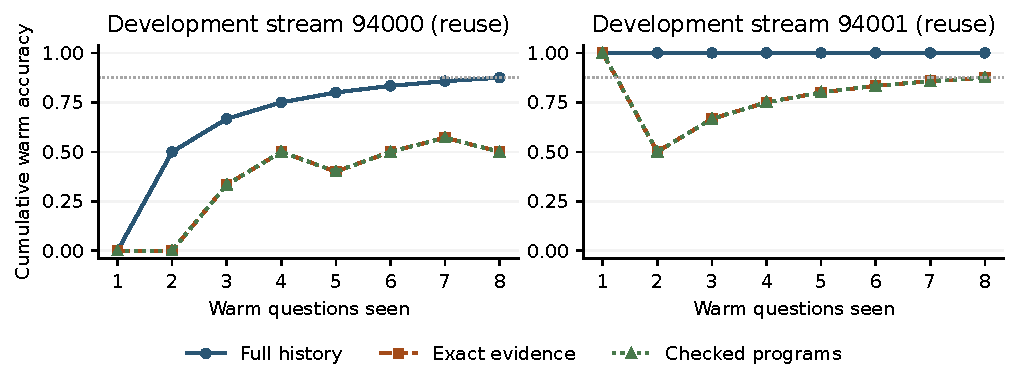
\includegraphics[width=.92\textwidth]{gh200_warm.pdf}
\caption{Cumulative accuracy over the eight warm questions in each adaptive
development stream. The horizontal line marks the final qualification threshold,
not a requirement at every prefix. These curves establish neither stateful gain
against reset memory nor transfer to fresh instances.}
\label{fig:gh200warm}
\end{figure*}

The follow-up stops at its deadline with 66 saved records out of 144 planned,
including one interrupted program-arm episode; 65 records complete. It uses
174 generation attempts and 780,757 known tokens. The interrupted call has
unknown usage, so the token total is incomplete and the receipt does not mark
usage verified. Recorded time is 2700.024 seconds: incremental export exceeds
the 2700-second ceiling by .024 seconds, and the receipt marks that cap
unsatisfied. Neither later old-panel nor final-panel evaluation occurs. Five
relations are admitted, but none executes through the checked \code{USE}/\code{COMPOSE}
path on a future question.
The intended execution mechanism is not demonstrated, and retention is
unassessed; missing panels are not zero-regression evidence.

Across both studies, resource expenditure is 235 calls, 947,781 known tokens
plus one unmeasured call, and 3277.40 study seconds. Accuracy is not pooled
across these adaptively changed configurations. The aggregate allowance is
3600 seconds, 4M tokens and 1800 attempts; exact compliance with the token
allowance is not asserted with missing usage. No further model-task attempt is
made in this phase, and reserved heldout seeds remain unused. Source hashes are
unchanged. Source-bound replay verifies 65 complete follow-up traces and 110
recorded SQL executions, separately identifying the partial trace. This is a
partial-study audit, not completion of the experimental protocol.

\paragraph{What the repair actually changes.}
On the follow-up total-refunds task, the first wrapper repeats a physical-table
subquery and aliases it as \code{reused}, shadowing the learned CTE.
Reconstruction returns 2311.75, but emptying the learned relation still returns
2311.75, so admission is rejected. The next proposal reads the actual
\code{reused} relation: reconstruction remains 2311.75 and the intervention
returns zero. It is admitted after four charged check SELECTs plus the ordinary
query. This is model-driven defect repair on one candidate, not later transfer.

Applicability is a distinct failure. The North-customer relation stores a guard
requiring the old customer count, six. A later proposed composition observes
three; a frozen old-panel count question observes four. Both guards reject
before the relation executes. The old-panel episode nevertheless answers
correctly with the guard's fresh count as its only current SQL result. This
records useful source-query reuse, without a counterfactual establishing the
answer's causal dependence on that result. Zero proposed-relation executions
therefore does not mean zero memory influence. The attempted composition also
contains an unsupported substitution placeholder; its validity is unestablished.

Finally, the old panel exposes stale scalar replay. History, evidence and
programs answer without SQL on two, six and four questions respectively; zero,
one and one of those answers are correct. The interface changes rows without
exposing a snapshot identifier, while reusing question text and schema. This
makes freshness an interface as well as a memory issue. Exact retained results
and a successful warm gate do not ensure fresh-instance competence, and no
paired intervention here isolates one cause of these failures.
